\documentclass[10pt, aspectratio=169, compress]{beamer}
\usetheme[progressbar=frame title, numbering=fraction]{metropolis}      % Use metropolis theme 
\setbeamertemplate{section in toc}[sections numbered]
\setbeamertemplate{subsection in toc}[subsections numbered]
\useoutertheme[subsection=false]{miniframes}
\setbeamercolor{section in head/foot}{fg=white, bg=mDarkTeal}
\setbeamercolor{background canvas}{bg=white}
\setbeamerfont{section in head/foot}{series=\bfseries}

\usefonttheme[onlymath]{serif}
\usepackage{amsmath}
\usepackage{remreset}
\usepackage{ragged2e}
\usepackage{booktabs}
\usepackage{makecell}
\usepackage{float}
\usepackage{subfig}
\usepackage{epigraph}
\usepackage{tikz}
\usetikzlibrary{positioning,calc,trees}
\usepackage[flushleft]{threeparttable}	% 3 part table 
\usepackage[justification=centering]{caption}
\captionsetup{skip=0pt}
\graphicspath{{./fig/}}

% Alterted itemize
\newenvironment{alerteditemize}{\begin{itemize}[<+-| alert@+>]}{\end{itemize}}

\makeatletter
\let\beamer@writeslidentry@miniframeson=\beamer@writeslidentry
\def\beamer@writeslidentry@miniframesoff{%
	\expandafter\beamer@ifempty\expandafter{\beamer@framestartpage}{}% does not happen normally
	{%else
		% removed \addtocontents commands
		\clearpage\beamer@notesactions%
	}
}
\newcommand*{\miniframeson}{\let\beamer@writeslidentry=\beamer@writeslidentry@miniframeson}
\newcommand*{\miniframesoff}{\let\beamer@writeslidentry=\beamer@writeslidentry@miniframesoff}
\beamer@compresstrue
\makeatother

%==============================================================
% Title Page
%==============================================================
%Information to be included in the title page:
\title{Análisis de Datos}
\subtitle{Construcción de Datos}
\author{Rony Rodriguez-Ramírez} 
\institute{LAMBDA}
\titlegraphic{\hfill
\includegraphics[height=1.5cm]{dime}}
\date{\today}
%==============================================================
\begin{document}
%------------------------------------------------	
\begin{frame}[plain]
	\maketitle 
\end{frame}
%------------------------------------------------
\section{Construcción de Datos}
%-----------------------------------------------
\subsection{Construcción de Datos}
%-----------------------------------------------
\begin{frame}{Desglose de tareas de trabajo de datos}
	\begin{itemize}
		\item Dividimos el proceso de trabajo de datos en cuatro etapas:
		\begin{enumerate}
			\item De-identificación
			\item Limpieza de datos
			\item Construcción de variables
			\item Análisis de datos
		\end{enumerate}
		\item Cada una de estas etapas tiene entradas y salidas bien definidas.
		\item Para cada etapa, debe haber una carpeta de códigos y un conjunto de datos correspondiente
		\item Los nombres de códigos, conjuntos de datos y salidas para cada etapa deben ser consistentes
		\item El código, los datos y los resultados de cada una de estas etapas deben pasar por al menos una ronda de revisión de código.
	\end{itemize}
\end{frame}
%-----------------------------------------------
\begin{frame}[t]{¿Qué es la construcción de datos?}
	\begin{itemize}
		\item La construcción de variables significa procesar los puntos de datos tal como se proporcionan en los datos sin procesar para que sean adecuados para el análisis
		\item Es en esta etapa que los datos sin procesar se transforman en datos de análisis.
		\item Esto se hace mediante la creación de variables derivadas (p. Ej., Dummies, índices, interacciones).
	\end{itemize}
\end{frame}
%-----------------------------------------------
\begin{frame}[t]{¿Qué es la construcción de datos?}
	\begin{itemize}
		\item Esto se hace mediante la creación de variables derivadas (p. Ej., Dummies, índices, interacciones).
		\item Es la única etapa en la que se realizarán cambios en los puntos de datos.
		\item La construcción está estrechamente relacionada con el diseño de investigación y el diseño de cuestionarios.
		\item Idealmente, la construcción del indicador debe realizarse justo después de la limpieza de datos, de acuerdo con el plan de pre-análisis. 
	\end{itemize}
\end{frame}
%-----------------------------------------------
\begin{frame}[t]{¿Qué es la construcción de datos?}
	\begin{itemize}
		\item La construcción está estrechamente relacionada con el diseño de investigación y el diseño de cuestionarios.
		\item Idealmente, la construcción del indicador debe realizarse justo después de la limpieza de datos, de acuerdo con el plan de pre-análisis. 
		\item Aquí es cuando utilizará más el conocimiento de los datos que adquirió y la documentación que creó durante el paso de limpieza.
		\item A menudo es útil comenzar a buscar comparaciones y otra documentación fuera del editor de código
	\end{itemize}
\end{frame}
%-----------------------------------------------
\begin{frame}[t]{¿Qué es la construcción de datos?}
	\begin{itemize}
		\item Inputs:
		\begin{itemize}
			\item Una o más bases de datos limpias. 
			\item Master data. 
		\end{itemize}
		\item Outputs:
		\begin{itemize}
			\item Una o más base de datos para análisis.
			\item Un \texttt{codebook} para cada base de datos para análisis.
		\end{itemize}
		\item Tareas: 
		\begin{itemize}
			\item Unidad de observación (en la encuesta) $\longrightarrow$ Unidad de análisis.
			\item Pregunta de la encuesta $\longrightarrow$ Indicador de análisis.
		\end{itemize}
	\end{itemize}
\end{frame}
%-----------------------------------------------
\begin{frame}{¿Por qué la construcción es una tarea separada de la limpieza de datos?}
	\begin{enumerate}
		\item Para diferenciar claramente los datos recopilados originalmente del resultado de las decisiones de procesamiento de datos
		\item Para garantizar que la definición de variable sea coherente en todas las fuentes de datos.
		\begin{itemize}
			\item Durante la limpieza de datos, creamos un output por cada input,
			\item Durante la construcción de datos, podemos tener múltiples entradas y salidas.
			\item Por ejemplo, podemos tener varias rondas de recopilación de datos que se limpiarán por separado, pero queremos que todas se construyan de la misma manera.
		\end{itemize}
	\end{enumerate}
\end{frame}
%-----------------------------------------------
\begin{frame}{¿Qué planear con anticipación?}
	\begin{itemize}
		\item ¿Cuáles son los indicadores finales necesarios para responder una pregunta de investigación?
		\item ¿Cómo se definen y calculan?
		\item ¿Cuáles son los pasos para llegar allí?
		\item ¿Cómo lidiar con diferentes rondas de recopilación de datos? 
	\end{itemize}
\end{frame}
%-----------------------------------------------
\begin{frame}{¿Por qué la construcción es una tarea separada de la limpieza de datos?}
	\begin{itemize}
		\item En la práctica, la construcción de datos a menudo ocurre al mismo tiempo que el análisis de datos.
		\item A medida que analiza los datos, serán necesarias diferentes variables construidas, así como subconjuntos y otras alteraciones de los datos.
		\item Sin embargo, incluso si la construcción termina antes del análisis solo en el orden en que se ejecuta el código, es importante considerarlos como pasos diferentes
	\end{itemize}
\end{frame}
%-----------------------------------------------
\section{Construyendo variables analíticas}
\subsection{Construyendo variables analíticas}
%-----------------------------------------------
\begin{frame}{Creando nuevas variables}
	\begin{itemize}
		\item Crear nuevas variables en lugar de sobrescribir la información original.
		\item Las variables construidas deben tener nombres intuitivos y funcionales.
		\item Ordene el conjunto de datos de modo que las variables relacionadas estén cercanas entre sí
	\end{itemize}
\end{frame}
%-----------------------------------------------
\begin{frame}{Abordar los valores atípicos}
	Durante la construcción, abordará los problemas que observó en los datos durante la limpieza, incluidos valores atípicos y valores faltantes: 
	\begin{itemize}[<+->]
		\item Lo único que no desea hacer es dejar una observación completa debido a valores atípicos
		\item Las formas comunes de abordar los valores atípicos son los recortes y la victoria.
	\end{itemize}
\end{frame}
%-----------------------------------------------
\begin{frame}[<+->]{Abordar los valores atípicos}
	Cómo tratar los valores atípicos e imputar valores perdidos son preguntas de investigación, pero hay algunas cosas a tener en cuenta.
	\begin{itemize}
		\item Asegúrese de documentar cuál fue el enfoque elegido por el equipo y por qué decidió usarlo en un caso particular
		\item Estas decisiones pueden afectar la distribución de variables y los resultados observados, por lo tanto, mantenga la variable original en el conjunto de datos en lugar de reemplazarla.
	\end{itemize}
\end{frame}
%-----------------------------------------------
\begin{frame}[<+->]{Unidades estandarizadas}
	Asegúrese de que haya coherencia entre las variables construidas:
	\begin{itemize}
		\item Recomendamos codificar preguntas sí/no como 1 y 0 o TRUE y FALSE, para que puedan usarse numéricamente como frecuencias en medias y como variables dummies en regresiones.
		\item Para las variables categóricas no binarias, verifique que las etiquetas y los niveles tengan la misma correspondencia entre las variables que usan las mismas opciones.
		\item Las variables numéricas que se comparan o agregan deben convertirse a la misma escala o unidad de medida
		\item Cuando convierta unidades, establezca las tasas de conversión en el archivo maestro do usando globals.
	\end{itemize}
\end{frame}
%-----------------------------------------------
\begin{frame}[<+->]{Crear medidas agregadas}
	\begin{itemize}
		\item El caso más simple de nuevas variables a crear son los indicadores agregados.
		\item Saltar al paso donde realmente crea estas variables parece intuitivo, pero también puede causarle muchos problemas, ya que pasar por alto los detalles puede afectar sus resultados
		\item Es importante verificar y volver a verificar las asignaciones de valores de las preguntas, así como sus escalas, antes de construir nuevas variables basadas en ellas.
		\item Observe las distribuciones de las variables originales y construidas.
	\end{itemize}
\end{frame}
%-----------------------------------------------
\begin{frame}{Crear medidas agregadas}
	\begin{itemize}
		\item Muchas veces es más fácil lidiar con conjuntos de datos largos al agregar
		\item Tenga en cuenta cómo se tratan los valores perdidos.
	\end{itemize}
\end{frame}
%-----------------------------------------------
\begin{frame}{Crear medidas agregadas}
	En Stata, los diferentes comandos tratan las faltas de manera diferente:
	\begin{itemize}
		\item gen income\_total = income\_wage + income\_rent + income\_sales
		\item egen income\_total = rowtotal(income\_wage income\_rent income\_sales)
		\item egen income\_total = rowtotal(income\_wage income\_rent
		income sales), m
		\item collapse (sum) income\_wage\_hh = income\_wage
		\item collapse (mean) income\_wage\_hh\_mean = income\_wage
		\item collapse (median) income\_wage\_hh\_median = income\_wage
	\end{itemize}
\end{frame}
%-----------------------------------------------
\begin{frame}{Merging base de datos}
	\begin{itemize}
		\item La fusión puede cambiar tanto el número de observaciones como el valor de las variables.
		\item Tenga cuidado al combinar conjuntos de datos que no tienen los mismos identificadores.
		\item Stata y R tratan los valores en conflicto de manera diferente: R crea dos variables y Stata mantiene las entradas del conjunto de datos maestros.
	\end{itemize}
\end{frame}
%-----------------------------------------------
\begin{frame}{Merging base de datos}
	\begin{figure}[H]
		\centering
		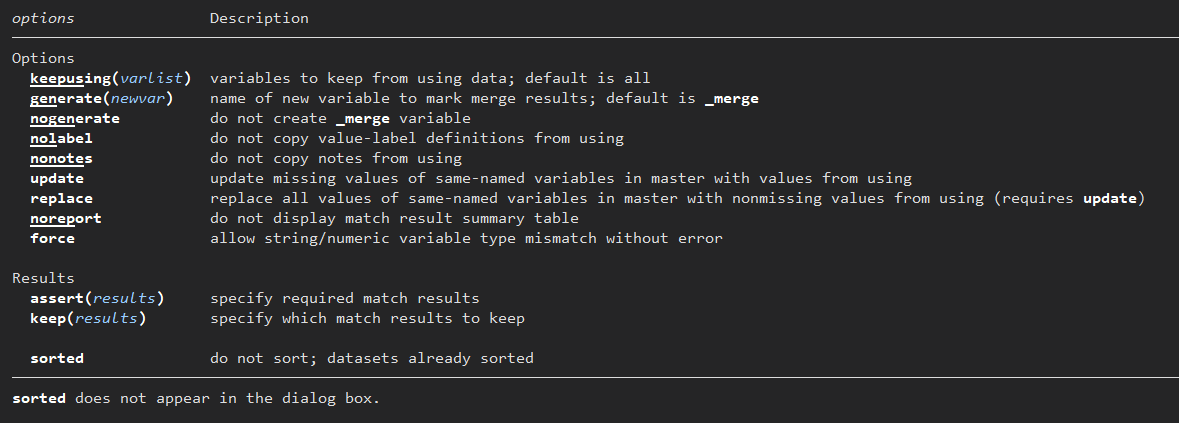
\includegraphics[width=1\textwidth]{merge.png}
	\end{figure}
\end{frame}
%-----------------------------------------------
\begin{frame}{Reshaping observaciones}
	\begin{itemize}
		\item La remodelación cambia la unidad de observación
		\item En Stata, la remodelación tiene una sintaxis muy única.
		\item Debe tener variables de identificación en el conjunto de datos para poder remodelarlo
		\item La remodelación creará observaciones en el conjunto de datos largo incluso cuando faltan variables		
	\end{itemize}
\end{frame}
%-----------------------------------------------
\begin{frame}{¿Qué son datos \textbf{tidy}?}
	\epigraph{Todas las familias felices se parecen unas a otras, pero cada familia infeliz lo es a su manera}{León Tolstói (Ana Karenina)}

	``Al igual que las familias, las base de datos tidy son todos iguales, pero cada base es desordenada a su manera. Los datos tidy proporcionan una forma estandarizada de vincular la estructura de una base de datos (su diseño físico) con su semántica (su significado)'' (Wickham, p. 2).
\end{frame}
%-----------------------------------------------
\begin{frame}{¿Qué son datos \textbf{tidy}?}
	\begin{itemize}
		\item Los datos tidy son una forma estándar de mapear el significado de un conjunto de datos a su estructura. 
		\item Los datos son desordenados o ordenados dependiendo de cómo las filas, columnas y tablas se combinan con observaciones, variables y tipos.
		\begin{enumerate}
			\item Cada variable forma una columna;
			\item Cada observación forma una fila; 
			\item Cada tipo de unidad de observación forma una tabla.
		\end{enumerate}
	\end{itemize}
\end{frame}
%-----------------------------------------------
\section{Previniendo errores}
\subsection{Previniendo errores}
%-----------------------------------------------
\begin{frame}{Previniendo errores}
	\begin{itemize}
		\item Las tareas de construcción más complejas implican cambiar la estructura de los datos, como la muestra y la unidad de observación.
		\item Las fusiones, remodelaciones y colapsos pueden cambiar el número de observaciones y crear entradas faltantes.
		\item Asegúrese de leer acerca de cómo cada comando trata las observaciones faltantes
		\item Si está subconjustando sus datos, elimine las observaciones explícitamente, indicando por qué lo está haciendo y cómo cambió el conjunto de datos
	\end{itemize}
\end{frame}
%-----------------------------------------------
\begin{frame}{Escribir \texttt{pseudocódigo}}
	\begin{itemize}
		\item Describa los pasos para crear su indicador en español simple.
		\item Refinar los subpasos involucrados.
		\item Cuando entres en demasiados detalles, escribe el código.
		\item Piense en los posibles errores que pueden aparecer en cada subpaso.
	\end{itemize}
\end{frame}
%-----------------------------------------------
\begin{frame}{Escribir \texttt{pesudocódigo}: Piense en los resultados esperados}
	\begin{itemize}
		\item Piense en cómo el comando que está usando trata los valores perdidos.
		\item Intenta predecir el resultado que obtendrás.
		\begin{itemize}
			\item ¿Se fusionarán todas las observaciones?
			\item ¿Cambiará el número de observaciones?
			\item ¿Se crearán los valores faltantes?
		\end{itemize}
	\end{itemize}
\end{frame}
%-----------------------------------------------
\begin{frame}{Documente los resultados observados}
	\begin{itemize}
		\item Explore los resultados reales de la operación.
		\item Escriba en los comentarios lo que sucedió.
		\item Agregue comentarios al código explicando consecuencias inesperadas
	\end{itemize}
\end{frame}

%-----------------------------------------------
\begin{frame}{Construya checks en su código}
	\begin{itemize}
		\item Probar la unidad de observación y la variable ID
		\item Lanzar mensajes de error o romper el código si
		\begin{itemize}
			\item Confirme los resultados esperados.
			\item Compruebe si las salidas están cambiando cuando vuelva a ejecutar el código
		\end{itemize}
		\item Use assert en Stata.
	\end{itemize}
\end{frame}
%-----------------------------------------------
\section{Outputs de construcción}
\subsection{Outputs de construcción}
%-----------------------------------------------
\begin{frame}{Base de datos construídas}
	\begin{itemize}
		\item Un conjunto de datos construido está construido para responder una pregunta de análisis;
		\item Diferentes piezas de análisis pueden requerir diferentes muestras o diferentes unidades de observación;
		\item Puede tener tantos conjuntos de datos construidos como sea necesario para el análisis;
		\item No se preocupe si no puede crear un único conjunto de datos de análisis "canónico";
		\item Si tiene varios conjuntos de datos construidos, asígneles un nombre cuidadoso para saber cuándo usarlos.
	\end{itemize}
\end{frame}
%-----------------------------------------------
\begin{frame}[<+->]{Documentar el output}
	\begin{itemize}
		\item La documentación es una salida de construcción tan relevante como el código y los datos.
		\item Alguien que no esté familiarizado con el proyecto debe poder comprender el contenido de los conjuntos de datos de análisis y los pasos dados para crearlos.
		\item La construcción de datos implica la traducción de puntos de datos concretos a mediciones más abstractas.
	\end{itemize}
\end{frame}
%-----------------------------------------------
\begin{frame}[<+->]{Documentar el output}
	\begin{itemize}
		\item Documente exactamente cómo se deriva o calcula cada variable
		\item Registre cuidadosamente cómo se combinaron, recodificaron y escalaron variables específicas, y haga referencia a esos registros en el código
		\item Esto puede ser parte de una discusión más amplia con su equipo sobre la creación de protocolos para la definición variable, lo que garantizará que los indicadores se definan de manera consistente en todos los proyectos.
	\end{itemize}
\end{frame}
%==============================================================
% Stata TIME
%==============================================================
\miniframesoff 	

\begin{frame}[plain, noframenumbering]
	\begin{center}
	\LARGE STATA TIME
		\begin{figure}[H]
			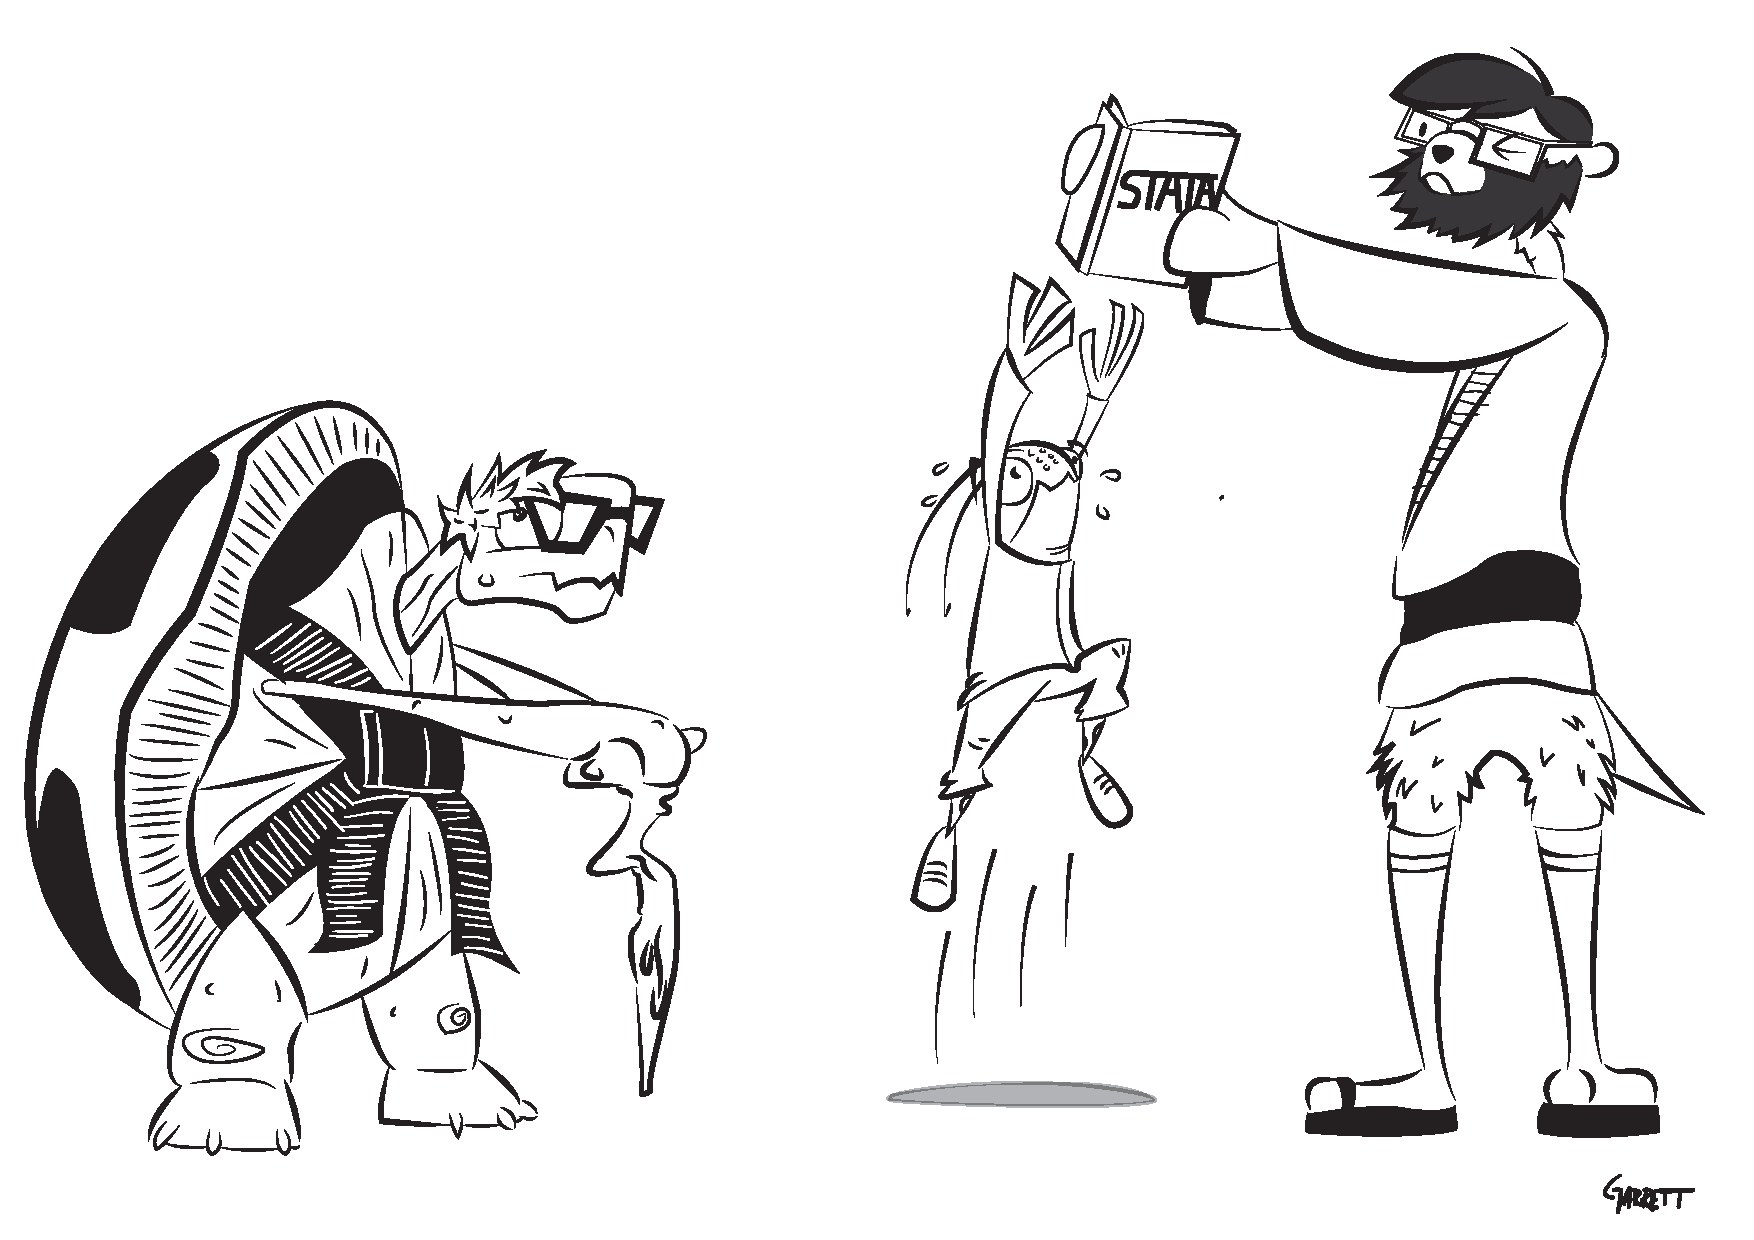
\includegraphics[width=0.57\textwidth]{stata.pdf}
		\end{figure}
	\end{center}
\end{frame}
%==============================================================
% END
%==============================================================	
\begin{frame}[plain, standout]
	Hasta la próxima semana.
\end{frame}
%-----------------------------------------------
\end{document}		
